\documentclass[11pt]{article}
\usepackage[a4paper,margin=20mm,headsep=6mm]{geometry}
\usepackage{amsmath,amssymb}
\usepackage[T1]{fontenc}
\usepackage{lmodern}
\usepackage{xcolor}
\usepackage{tikz}
\usetikzlibrary{arrows.meta}
\usepackage[most]{tcolorbox}
\usepackage{enumitem}
\usepackage{fancyhdr}
\usepackage{needspace}
\usepackage{lastpage}
\definecolor{chalk}{HTML}{2F6F8F}
\definecolor{chalkdk}{HTML}{24576F}
\definecolor{amber}{HTML}{D98A3D}
\definecolor{ink}{HTML}{1A2B34}
\definecolor{inksoft}{HTML}{4A5F68}
\definecolor{paper}{HTML}{F6F4EF}
\definecolor{line}{HTML}{DFE3E0}
\color{ink}
\setlength{\parindent}{0pt}
\setlength{\parskip}{4pt}
\pagestyle{fancy}
\fancyhf{}
\renewcommand{\headrulewidth}{0.4pt}
\renewcommand{\headrule}{\hbox to\headwidth{\color{line}\leaders\hrule height 0.4pt\hfill}}
\lhead{\small\color{inksoft}\textsc{Chapter 3F--3L : Exponentials \& Logarithms}}
\rhead{\small\color{inksoft}Year 10 Methods : Question Booklet}
\cfoot{\small\color{inksoft}Page \thepage\ of \pageref{LastPage}}
\newcommand{\sectionband}[3]{%
  \needspace{5\baselineskip}\vspace{6pt}
  \begin{tcolorbox}[enhanced,colback=chalk,colframe=chalk,boxrule=0pt,left=12pt,right=12pt,top=8pt,bottom=8pt,arc=4pt,
      overlay={\node[anchor=east,text=white,opacity=0.9] at ([xshift=-12pt]frame.east) {\small\textsf{#3}};}]
    {\color{white}\large\bfseries\textsf{#1}\quad #2}
  \end{tcolorbox}}
\newtcolorbox{refbox}{enhanced,breakable,colback=paper,colframe=line,boxrule=0.6pt,left=12pt,right=12pt,top=8pt,bottom=8pt,arc=3pt}
\newtcolorbox{workedbox}{enhanced,colback=chalk!6,colframe=chalk!55,boxrule=0.7pt,left=12pt,right=12pt,top=8pt,bottom=8pt,arc=3pt,borderline west={3pt}{0pt}{chalk}}
\newcommand{\worklines}[1]{\par\vspace{2pt}\foreach \n in {1,...,#1}{\vspace{9pt}\noindent\textcolor{line!140!white}{\rule{\linewidth}{0.3pt}}\par}\vspace{2pt}}
% one hurdle question: kept on a single page with its figure and working space
\newenvironment{hq}{\begin{minipage}[t]{\linewidth}\setlength{\parskip}{4pt}}{\end{minipage}}
\tikzset{figstyle/.style={line join=round,>=Stealth}}
% ---- Figure macros (schematic, not to scale) ----
% Exponential graph on axes.
% #1 xmin #2 xmax #3 ymin #4 ymax #5 clipped plots #6 unclipped labels
\newcommand{\expfig}[6]{\begin{center}\begin{tikzpicture}[figstyle,x=0.72cm,y=0.3cm]
  \draw[chalkdk!45,->](#1-0.3,0)--(#2+0.45,0)node[right,font=\scriptsize]{$x$};
  \draw[chalkdk!45,->](0,#3-0.4)--(0,#4+0.7)node[above,font=\scriptsize]{$y$};
  \begin{scope}\clip(#1-0.3,#3-0.4)rectangle(#2+0.3,#4+0.4);
  #5
  \end{scope}
  #6
\end{tikzpicture}\end{center}}
% dashed asymptote across an \expfig: #1 y-value #2 xmin #3 xmax
\newcommand{\asym}[3]{\draw[amber,dashed,thick](#2-0.3,#1)--(#3+0.3,#1);}
% exponential curve: #1 pgf expression in \x, #2 xmin, #3 xmax, #4 colour
\newcommand{\expcurve}[4]{\draw[#4,very thick,domain=#2:#3,samples=120,smooth]plot(\x,{#1});}
% labelled point
\newcommand{\pt}[3]{\fill[chalkdk](#1)circle(2pt);\node[font=\scriptsize,#2]at(#1){#3};}
% Blank sketching grid: x from -3 to 3, y from #1 to #2 (square cells)
\newcommand{\sketchgrid}[2]{\par\vspace{2pt}\begin{center}\begin{tikzpicture}[x=0.7cm,y=0.35cm]
  \draw[xstep=0.5,ystep=1,line!120!white,very thin](-3.5,#1)grid(3.5,#2);
  \draw[chalk,->](-3.6,0)--(3.8,0)node[right,font=\small,ink]{$x$};
  \draw[chalk,->](0,#1-0.2)--(0,#2+0.6)node[above,font=\small,ink]{$y$};
  \foreach \x in {-3,...,3}{\ifnum\x=0\else\draw[chalkdk](\x,-0.15)--(\x,0.15)node[below=3pt,font=\scriptsize,ink]{$\x$};\fi}
  \foreach \y in {#1,...,#2}{\ifodd\y\else\ifnum\y=0\else\draw[chalkdk](-0.07,\y)--(0.07,\y)node[left=2pt,font=\scriptsize,ink]{$\y$};\fi\fi}
\end{tikzpicture}\end{center}}
% Growth / decay curves (schematic). #1 initial label #2 rule label #3 horizontal var #4 vertical var #5 extras
\newcommand{\figGrowth}[5]{\begin{center}\begin{tikzpicture}[figstyle,x=0.82cm,y=0.72cm]
  \draw[chalkdk!50,->](0,0)--(5.6,0)node[right,font=\scriptsize]{#3};
  \draw[chalkdk!50,->](0,0)--(0,3.6)node[above,font=\scriptsize]{#4};
  \draw[chalkdk,very thick,domain=0:5,samples=60,smooth]plot(\x,{0.8*1.32^\x});
  \fill[chalkdk](0,0.8)circle(2pt);\node[font=\scriptsize,left]at(0,0.8){#1};
  \node[font=\small,chalkdk,anchor=west]at(0.35,3.1){#2};
  #5
\end{tikzpicture}\end{center}}
\newcommand{\figDecay}[5]{\begin{center}\begin{tikzpicture}[figstyle,x=0.82cm,y=0.72cm]
  \draw[chalkdk!50,->](0,0)--(5.6,0)node[right,font=\scriptsize]{#3};
  \draw[chalkdk!50,->](0,0)--(0,3.3)node[above,font=\scriptsize]{#4};
  \draw[chalkdk,very thick,domain=0:5,samples=60,smooth]plot(\x,{2.6*0.72^\x});
  \fill[chalkdk](0,2.6)circle(2pt);\node[font=\scriptsize,left]at(0,2.6){#1};
  \node[font=\small,chalkdk,anchor=west]at(1.5,2.55){#2};
  #5
\end{tikzpicture}\end{center}}
% marked point / target line on the growth and decay curves
\newcommand{\growthpt}[1]{\draw[amber,dashed](3,0)--(3,1.84)--(0,1.84);\fill[amber](3,1.84)circle(2pt);\node[font=\scriptsize,right]at(3.05,1.75){#1};}
\newcommand{\growthtarget}[3]{\pgfmathsetmacro{\gy}{0.8*#3}\pgfmathsetmacro{\gx}{ln(#3)/ln(1.32)}%
  \draw[amber,dashed,thick](0,\gy)--(5.2,\gy)node[right,font=\scriptsize,amber!80!black]{#1};
  \draw[amber,dashed](\gx,\gy)--(\gx,0)node[below,font=\scriptsize,ink]{#2};\fill[amber](\gx,\gy)circle(2pt);}
\newcommand{\decaypt}[1]{\draw[amber,dashed](3,0)--(3,0.97)--(0,0.97);\fill[amber](3,0.97)circle(2pt);\node[font=\scriptsize,above right]at(3,0.97){#1};}
\newcommand{\decaytarget}[3]{\pgfmathsetmacro{\dy}{2.6*#3}\pgfmathsetmacro{\dx}{ln(#3)/ln(0.72)}%
  \draw[amber,dashed,thick](0,\dy)--(5.2,\dy)node[right,font=\scriptsize,amber!80!black]{#1};
  \draw[amber,dashed](\dx,\dy)--(\dx,0)node[below,font=\scriptsize,ink]{#2};\fill[amber](\dx,\dy)circle(2pt);}
% Compounding timeline. #1 principal #2 multiplier per period #3 last period label #4 period word
\newcommand{\figCompound}[4]{\begin{center}\begin{tikzpicture}[figstyle,x=1cm,y=1cm,font=\small]
  \draw[chalkdk,thick](0,0)--(4.5,0);\draw[chalkdk,thick,dotted](4.5,0)--(5.6,0);\draw[chalkdk,thick,->](5.6,0)--(6.9,0)node[right,font=\scriptsize]{#4};
  \foreach \x/\l in {0/0,1.4/1,2.8/2,4.2/3,6.3/{#3}}{\draw[chalkdk](\x,-0.12)--(\x,0.12);\node[below,font=\scriptsize]at(\x,-0.12){$\l$};}
  \foreach \a/\b in {0/1.4,1.4/2.8,2.8/4.2}{\draw[amber,thick,->]([yshift=4pt]\a,0.1) to[bend left=50] ([yshift=4pt]\b,0.1);\node[font=\scriptsize,amber!80!black]at({(\a+\b)/2},0.85){$\times#2$};}
  \node[font=\scriptsize,chalkdk]at(0,-0.75){#1};\node[font=\scriptsize,chalkdk]at(6.3,-0.75){$A=\,?$};
\end{tikzpicture}\end{center}}
% Log form <-> index form. #1 base #2 power (the log) #3 number
\newcommand{\figLogForm}[3]{\begin{center}\begin{tikzpicture}[figstyle,font=\normalsize]
  \node(L)at(0,0){$\log_{\textcolor{chalkdk}{#1}}#3=\textcolor{amber!85!black}{#2}$};
  \node(I)at(4.6,0){$\textcolor{chalkdk}{#1}^{\,\textcolor{amber!85!black}{#2}}=#3$};
  \draw[chalkdk!60,<->,thick](L.east)--(I.west)node[midway,above,font=\scriptsize,inksoft]{same fact};
  \node[font=\scriptsize,inksoft]at(0,-0.6){log form};\node[font=\scriptsize,inksoft]at(4.6,-0.6){index form};
  \node[font=\scriptsize,amber!80!black]at(2.3,-1.05){the log is the \textbf{power}};
\end{tikzpicture}\end{center}}
% Log-scale number line. #1 min #2 max #3 posA #4 labelA #5 posB #6 labelB #7 scale name
\newcommand{\figLogLine}[7]{\begin{center}\begin{tikzpicture}[figstyle,x=0.72cm,y=1cm]
  \draw[chalkdk,thick](#1-0.4,0)--(#2+0.4,0);
  \foreach \k in {#1,...,#2}{\draw[chalkdk](\k,-0.1)--(\k,0.1);\node[below,font=\scriptsize]at(\k,-0.1){$\k$};}
  \node[font=\scriptsize,inksoft,anchor=west]at(#2+0.5,0){#7};
  \fill[amber](#3,0)circle(2.6pt);\node[font=\scriptsize,above=4pt,chalkdk]at(#3,0){#4};
  \fill[amber](#5,0)circle(2.6pt);\node[font=\scriptsize,above=4pt,chalkdk]at(#5,0){#6};
  \pgfmathsetmacro{\lo}{min(#3,#5)}\pgfmathsetmacro{\hi}{max(#3,#5)}\draw[amber!85!black,thick,<->]([yshift=-15pt]\lo,0) to[bend right=22] node[midway,below,font=\scriptsize]{$\times\,?$} ([yshift=-15pt]\hi,0);
\end{tikzpicture}\end{center}}
% Logarithmic bar chart. #1 list name/value #2 vertical axis label #3 axis max
\newcommand{\figLogBars}[3]{\begin{center}\begin{tikzpicture}[figstyle,x=1.1cm,y=0.42cm]
  \foreach \y in {1,...,#3}{\draw[line!120!white,very thin](0.3,\y)--(6.2,\y);\node[left,font=\scriptsize]at(0.3,\y){$\y$};}
  \draw[chalkdk!60](0.3,0)--(6.2,0);\draw[chalkdk!60,->](0.3,0)--(0.3,#3+0.8)node[above,font=\scriptsize]{#2};
  \foreach \n/\v [count=\i] in {#1}{\fill[chalk!75](\i-0.28,0)rectangle(\i+0.28,\v);\node[above,font=\scriptsize]at(\i,\v){$\v$};\node[below,font=\scriptsize]at(\i,0){\n};}
\end{tikzpicture}\end{center}}
% Grid for plotting log10 of a quantity against time. #1 tmax #2 ymax #3 vertical label #4 horizontal label #5 extras
\newcommand{\loggrid}[5]{\par\vspace{2pt}\begin{center}\begin{tikzpicture}[figstyle,x=1.1cm,y=0.58cm]
  \draw[xstep=0.5,ystep=0.5,line!120!white,very thin](0,0)grid(#1+0.5,#2+0.5);
  \draw[chalk,->](0,0)--(#1+0.8,0)node[right,font=\small,ink]{#4};
  \draw[chalk,->](0,0)--(0,#2+0.9)node[above,font=\small,ink]{#3};
  \foreach \t in {0,...,#1}{\draw[chalkdk](\t,-0.1)--(\t,0.1);\node[below,font=\scriptsize]at(\t,-0.1){$\t$};}
  \foreach \y in {1,...,#2}{\draw[chalkdk](-0.06,\y)--(0.06,\y);\node[left,font=\scriptsize]at(-0.06,\y){$\y$};}
  #5
\end{tikzpicture}\end{center}}
% y = a^x meeting y = b. #1 base (>1) #2 b #3 curve label #4 x label
\newcommand{\figIntersect}[4]{\pgfmathsetmacro{\xint}{ln(#2)/ln(#1)}\pgfmathsetmacro{\yu}{3.4/(1.3*#2)}%
  \pgfmathsetmacro{\xtop}{ln(1.3*#2)/ln(#1)}\pgfmathsetmacro{\xend}{\xint+1.4}%
  \begin{center}\begin{tikzpicture}[figstyle,x=0.8cm,y=\yu cm]
  \draw[chalkdk!45,->](-1.6,0)--(\xend+0.3,0)node[right,font=\scriptsize]{$x$};
  \draw[chalkdk!45,->](0,-0.06*#2)--(0,1.4*#2)node[above,font=\scriptsize]{$y$};
  \draw[amber,dashed,thick](-1.6,#2)--(\xend,#2)node[right,font=\scriptsize,amber!80!black]{$y=#2$};
  \draw[chalkdk,very thick,domain=-1.6:\xtop,samples=100,smooth]plot(\x,{#1^\x});
  \node[font=\scriptsize,chalkdk,left]at(\xtop-0.1,1.22*#2){#3};
  \draw[chalkdk,dashed](\xint,#2)--(\xint,0)node[below,font=\scriptsize,ink]{#4};
  \fill[amber](\xint,#2)circle(2.2pt);
\end{tikzpicture}\end{center}}
\begin{document}
\thispagestyle{empty}
\begin{tikzpicture}[remember picture,overlay]
  \fill[chalk] (current page.north west) rectangle ([yshift=-62mm]current page.north east);
  \node[anchor=north west,text=white,align=left] at ([xshift=20mm,yshift=-20mm]current page.north west)
    {{\Huge\bfseries\textsf{Chapter 3: Exponentials \& Logarithms}}\\[4mm]{\LARGE\textsf{Student Question Booklet}}\\[3mm]{\large\textsf{Sections 3F--3L : Year 10 Mathematical Methods : 2026}}};
\end{tikzpicture}
\vspace{58mm}

\vspace{6mm}
\begin{refbox}
{\bfseries\color{chalkdk}How to use this booklet}\\[2pt]
This booklet is your \textbf{map through sections 3F--3L} --- exponential graphs, growth and decay, compound interest and logarithms. For every section you will find:
\begin{itemize}[leftmargin=16pt,itemsep=2pt,topsep=3pt]
  \item \textbf{Worked examples} --- fully solved examples with a diagram where it helps, plus the matching textbook example numbers and pages to cross-reference.
  \item \textbf{Question sets} --- the questions to practise, grouped by \textit{Building Understanding}, \textit{Fluency}, \textit{Problem-solving}, \textit{Reasoning} and \textit{Enrichment}, with page numbers. Find them in your own textbook.
  \item \textbf{Hurdle questions} --- five questions you \textbf{must} be able to do to pass the section, with working space (and a grid wherever you need to sketch).
\end{itemize}
\vspace{2pt}{\small\color{inksoft}Diagrams are schematic (not to scale). Sections marked \textsf{10A} are extension. Your calculator's \textsf{log} button is base 10. Round as instructed and always show working --- write the rule before you calculate.}
\end{refbox}
\vspace{4mm}{\small\color{inksoft}Page references are to \emph{Essential Mathematics for the Victorian Curriculum 10 \& 10A}, 3rd ed. Question sets belong to the textbook; the worked examples, diagrams and hurdle questions are original material written for this course.}
\clearpage
\newpage
\quad
\clearpage

\sectionband{3F}{Exponential relations and their graphs}{CORE}

\begin{refbox}
{\bfseries\color{chalkdk}Textbook worked examples}\;\textcolor{inksoft}{\small(cross-reference in your textbook)}\\[3pt]
\begin{itemize}[leftmargin=16pt,itemsep=1pt,topsep=2pt]
  \item \textbf{Example 16} --- Sketching graphs of exponentials \textcolor{inksoft}{(p.\,251)}
  \item \textbf{Example 17} --- Sketching with reflections \textcolor{inksoft}{(p.\,252)}
  \item \textbf{Example 18} --- Solving exponential equations graphically \textcolor{inksoft}{(p.\,252)}
\end{itemize}
\vspace{4pt}{\bfseries\color{chalkdk}Question sets}\;\textcolor{inksoft}{\small(practise from your textbook)}\\[3pt]
\begin{itemize}[leftmargin=16pt,itemsep=1pt,topsep=2pt]
  \item \textbf{Building Understanding:} Q1--3 \textcolor{inksoft}{(p.\,250--251)}
  \item \textbf{Fluency:} Q1--4 \textcolor{inksoft}{(p.\,253)}
  \item \textbf{Problem-solving:} Q5--8 \textcolor{inksoft}{(p.\,253)}
  \item \textbf{Reasoning:} Q9--12 \textcolor{inksoft}{(p.\,254)}
  \item \textbf{Enrichment: $y=2^{-x}$ and $y=\left(\tfrac12\right)^{x}$:} Q13 \textcolor{inksoft}{(p.\,254)}
\end{itemize}\end{refbox}

\vspace{4pt}{\bfseries\color{chalkdk}\large Worked examples}\;\textcolor{inksoft}{\small(study the method, then try the hurdles)}\par

\begin{workedbox}

{\bfseries\color{chalkdk}Sketching an exponential graph}\par\vspace{3pt}

Sketch $y=3^x$. Label the $y$-intercept, the point where $x=1$, and the asymptote.\par\vspace{2pt}

\expfig{-3}{2.2}{-1}{9}{\asym{0}{-3}{2.2}\expcurve{3^\x}{-3}{2.05}{chalkdk}}{\pt{0,1}{above left=1pt}{$(0,1)$}\pt{1,3}{right=3pt}{$(1,3)$}\node[font=\scriptsize,amber!80!black,anchor=north west]at(0.15,-0.35){asymptote $y=0$};\node[font=\small,chalkdk,anchor=west]at(2.15,8.4){$y=3^x$};}

{\bfseries Solution.}\ Every graph $y=a^x$ (with $a>1$) passes through $(0,1)$ because $a^0=1$. At $x=1$, $y=3^1=3$, giving $(1,3)$. For negative $x$ the values get very small ($3^{-2}=\tfrac19$) but never reach $0$, so the $x$-axis, $y=0$, is the \textbf{asymptote}. The curve rises steeply for $x>0$.

\end{workedbox}

\begin{workedbox}

{\bfseries\color{chalkdk}Reflecting an exponential graph}\par\vspace{3pt}

On the same axes, sketch $y=2^{-x}$ and $y=-2^{x}$. State the reflection that produces each graph from $y=2^x$.\par\vspace{2pt}

\expfig{-3}{3}{-8}{8}{\asym{0}{-3}{3}\expcurve{0.5^\x}{-3}{3}{chalkdk}\expcurve{-(2^\x)}{-3}{3}{amber!85!black}}{\pt{0,1}{above right=1pt}{$(0,1)$}\pt{0,-1}{anchor=north east,inner sep=2pt}{$(0,-1)$}\node[font=\small,chalkdk,anchor=west]at(-2.2,7.4){$y=2^{-x}$};\node[font=\small,amber!85!black,anchor=east]at(2.5,-7.4){$y=-2^{x}$};}

{\bfseries Solution.}\ Replacing $x$ with $-x$ reflects the graph in the \textbf{$y$-axis}: $y=2^{-x}$ still passes through $(0,1)$ and has asymptote $y=0$, but it \emph{decreases}. Putting a negative in front, $y=-2^x$, reflects the graph in the \textbf{$x$-axis}: it passes through $(0,-1)$, keeps the asymptote $y=0$, and lies below it.

\end{workedbox}

\begin{workedbox}

{\bfseries\color{chalkdk}A translated exponential graph}\par\vspace{3pt}

For $y=2^x-4$, find the asymptote, the $y$-intercept and the $x$-intercept, then sketch the graph.\par\vspace{2pt}

\expfig{-3}{3}{-5}{4}{\asym{-4}{-3}{3}\expcurve{2^\x-4}{-3}{3}{chalkdk}}{\pt{0,-3}{anchor=south east,inner sep=2pt}{$(0,-3)$}\pt{2,0}{above left=1pt}{$(2,0)$}\node[font=\scriptsize,amber!80!black,anchor=north east]at(3.3,-4.15){$y=-4$};\node[font=\small,chalkdk,anchor=west]at(-2.9,2.6){$y=2^x-4$};}

{\bfseries Solution.}\ Subtracting $4$ moves the whole graph, \emph{including the asymptote}, down $4$: the asymptote is $y=-4$. When $x=0$, $y=1-4=-3$, so the $y$-intercept is $(0,-3)$. When $y=0$: \[ 2^x-4=0 \;\Rightarrow\; 2^x=4=2^2 \;\Rightarrow\; x=2, \] so the $x$-intercept is $(2,0)$.

\end{workedbox}
\newpage
\vspace{6pt}{\bfseries\color{amber}\large Hurdle questions --- Section 3F}\;\textcolor{inksoft}{\small(show all working)}\par\nopagebreak\vspace{2pt}

\begin{enumerate}[leftmargin=20pt,itemsep=8pt,topsep=4pt,beginpenalty=10000,label=\textbf{H\arabic*.}]

  \item \begin{hq}Sketch the graph of $y=4^x$ on the grid. Label the $y$-intercept, the point where $x=1$, and the asymptote.

\sketchgrid{-2}{8}

  \worklines{2}
  \end{hq}

  \item \begin{hq}On the same axes, sketch $y=3^{-x}$ and $y=-3^{x}$. Label each $y$-intercept and the asymptote, and state which axis each graph is a reflection of $y=3^x$ in.

\sketchgrid{-8}{8}

  \worklines{3}
  \end{hq}

  \item \begin{hq}For the graph of $y=2^x-8$, find: \textbf{(a)} the equation of the asymptote, \textbf{(b)} the $y$-intercept, \textbf{(c)} the $x$-intercept. Then sketch the graph, labelling all three features.

\sketchgrid{-9}{2}

  \worklines{2}
  \end{hq}

  \item \begin{hq}The graphs of $y=3^x$ and $y=27$ meet at one point. Find its coordinates \emph{without} a calculator, and explain your method using powers of $3$.

\figIntersect{3}{27}{$y=3^x$}{$x=\,?$}

  \worklines{2}
  \end{hq}

  \item \begin{hq}Explain why the equation $2^x=-4$ has no solution. Refer to the graph of $y=2^x$ and its asymptote in your answer.

\expfig{-3}{2.6}{-5}{6}{\asym{0}{-3}{2.6}\expcurve{2^\x}{-3}{2.6}{chalkdk}\draw[inksoft,dotted,thick](-3.3,-4)--(2.9,-4);}{\pt{0,1}{above left=1pt}{$(0,1)$}\node[font=\scriptsize,inksoft,anchor=west]at(0.15,-4.6){$y=-4$};\node[font=\small,chalkdk,anchor=west]at(2.65,6.0){$y=2^x$};}

  \worklines{3}
  \end{hq}

\end{enumerate}\clearpage

\sectionband{3G}{Exponential growth and decay}{CORE}

\begin{refbox}
{\bfseries\color{chalkdk}Textbook worked examples}\;\textcolor{inksoft}{\small(cross-reference in your textbook)}\\[3pt]
\begin{itemize}[leftmargin=16pt,itemsep=1pt,topsep=2pt]
  \item \textbf{Example 19} --- Writing exponential rules \textcolor{inksoft}{(p.\,258)}
  \item \textbf{Example 20} --- Applying exponential rules \textcolor{inksoft}{(p.\,258)}
\end{itemize}
\vspace{4pt}{\bfseries\color{chalkdk}Question sets}\;\textcolor{inksoft}{\small(practise from your textbook)}\\[3pt]
\begin{itemize}[leftmargin=16pt,itemsep=1pt,topsep=2pt]
  \item \textbf{Building Understanding:} Q1--3 \textcolor{inksoft}{(p.\,257)}
  \item \textbf{Fluency:} Q1--6 \textcolor{inksoft}{(p.\,259--260)}
  \item \textbf{Problem-solving:} Q7--9 \textcolor{inksoft}{(p.\,260--261)}
  \item \textbf{Reasoning:} Q10--11 \textcolor{inksoft}{(p.\,261)}
  \item \textbf{Enrichment: Half-life:} Q12--14 \textcolor{inksoft}{(p.\,261)}
\end{itemize}\end{refbox}

\vspace{4pt}{\bfseries\color{chalkdk}\large Worked examples}\;\textcolor{inksoft}{\small(study the method, then try the hurdles)}\par

\begin{workedbox}

{\bfseries\color{chalkdk}Writing growth and decay rules}\par\vspace{3pt}

Write a rule for each situation, defining your variables. \textbf{(a)} A colony of $500$ bacteria grows by $20\%$ every hour. \textbf{(b)} A swimming pool holding $12\,000$ L loses $5\%$ of its water each day.\par\vspace{2pt}

{\bfseries Solution.}\ Growing by $r\%$ means multiplying by $1+\tfrac{r}{100}$ each period; losing $r\%$ means multiplying by $1-\tfrac{r}{100}$. \begin{align*} \text{(a)}\;\; & N = \text{number of bacteria after } t \text{ hours:} && N=500(1.2)^t \quad(\text{growth, } \times1.2)\\ \text{(b)}\;\; & V = \text{volume in litres after } t \text{ days:} && V=12\,000(0.95)^t \quad(\text{decay, } \times0.95) \end{align*}

\end{workedbox}

\begin{workedbox}

{\bfseries\color{chalkdk}Applying a decay rule}\par\vspace{3pt}

A car bought for \$28\,000 loses $15\%$ of its value each year. Write a rule for its value and find the value after $4$ years, to the nearest dollar.\par\vspace{2pt}

\figDecay{$28\,000$}{$V=28\,000(0.85)^n$}{$n$ (years)}{$V$ (\$)}{\decaypt{$(4,\,?)$}}

{\bfseries Solution.}\ A $15\%$ loss each year means multiplying by $0.85$, so $V=28\,000(0.85)^n$. Substitute $n=4$: \[ V=28\,000\times0.85^4=28\,000\times0.52200625=14\,616.175\ldots \] After $4$ years the car is worth about \textbf{\$14\,616}.

\end{workedbox}
\newpage
\vspace{6pt}{\bfseries\color{amber}\large Hurdle questions --- Section 3G}\;\textcolor{inksoft}{\small(show all working)}\par\nopagebreak\vspace{2pt}

\begin{enumerate}[leftmargin=20pt,itemsep=8pt,topsep=4pt,beginpenalty=10000,label=\textbf{H\arabic*.}]

  \item \begin{hq}Write an exponential rule for each situation, defining your variables. \textbf{(a)} \$2500 grows by $6\%$ per year. \textbf{(b)} An $80$ g radioactive sample decays by $9\%$ per hour. \textbf{(c)} A population of $12\,000$ falls by $2.5\%$ per year.

  \worklines{5}
  \end{hq}

  \item \begin{hq}A town has $4500$ people and its population grows by $2\%$ per year. \textbf{(a)} Write a rule for the population $P$ after $n$ years. \textbf{(b)} Find the population after $10$ years, to the nearest whole person.

\figGrowth{$4500$}{$P=\;?$}{$n$ (years)}{$P$}{}

  \worklines{4}
  \end{hq}

  \item \begin{hq}A new phone costs \$1200 and loses $25\%$ of its value each year. Find its value after $3$ years.

\figDecay{$1200$}{$V=\;?$}{$n$ (years)}{$V$ (\$)}{\decaypt{$(3,\,?)$}}

  \worklines{4}
  \end{hq}

  \item \begin{hq}A water tank holding $20\,000$ L has a leak, and loses $4\%$ of its water each day. How much water is left after one week? Give your answer to the nearest litre.

\figDecay{$20\,000$}{$W=\;?$}{$t$ (days)}{$W$ (L)}{}

  \worklines{4}
  \end{hq}

  \item \begin{hq}For the town in H2, use your rule and a table of values (trial and error) to find the first whole number of years after which the population is more than $6000$.

\figGrowth{$4500$}{}{$n$ (years)}{$P$}{\growthtarget{$6000$}{$n=\,?$}{1.333}}

\begin{center}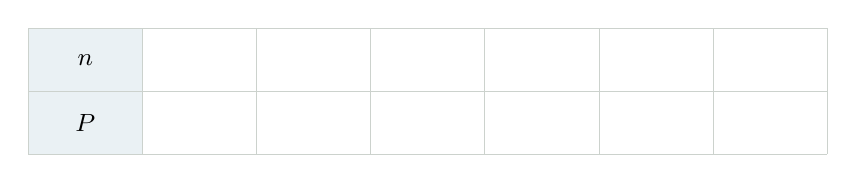
\begin{tikzpicture}[x=1.45cm,y=0.8cm,font=\small]
  \fill[chalk!10](0,0)rectangle(1,2);
  \draw[line!160!white,xstep=1,ystep=1](0,0)grid(7,2);
  \node at(0.5,1.5){$n$};\node at(0.5,0.5){$P$};
\end{tikzpicture}\end{center}

  \worklines{3}
  \end{hq}

\end{enumerate}\clearpage

\sectionband{3H}{Compound interest}{CORE}

\begin{refbox}
{\bfseries\color{chalkdk}Textbook worked examples}\;\textcolor{inksoft}{\small(cross-reference in your textbook)}\\[3pt]
\begin{itemize}[leftmargin=16pt,itemsep=1pt,topsep=2pt]
  \item \textbf{Example 21} --- Using the compound interest formula \textcolor{inksoft}{(p.\,264)}
  \item \textbf{Example 22} --- Converting rates and time periods \textcolor{inksoft}{(p.\,264)}
  \item \textbf{Example 23} --- Finding compounded amounts using months \textcolor{inksoft}{(p.\,265)}
\end{itemize}
\vspace{4pt}{\bfseries\color{chalkdk}Question sets}\;\textcolor{inksoft}{\small(practise from your textbook)}\\[3pt]
\begin{itemize}[leftmargin=16pt,itemsep=1pt,topsep=2pt]
  \item \textbf{Building Understanding:} Q1--4 \textcolor{inksoft}{(p.\,263)}
  \item \textbf{Fluency:} Q1--4 \textcolor{inksoft}{(p.\,265--266)}
  \item \textbf{Problem-solving:} Q5--7 \textcolor{inksoft}{(p.\,266)}
  \item \textbf{Reasoning:} Q8--9 \textcolor{inksoft}{(p.\,266)}
  \item \textbf{Enrichment: Double your money:} Q10 \textcolor{inksoft}{(p.\,266)}
\end{itemize}\end{refbox}

\vspace{4pt}{\bfseries\color{chalkdk}\large Worked examples}\;\textcolor{inksoft}{\small(study the method, then try the hurdles)}\par

\begin{workedbox}

{\bfseries\color{chalkdk}Using the compound interest formula}\par\vspace{3pt}

\$6000 is invested at $5\%$ p.a., compounded annually, for $4$ years. Find the final amount and the interest earned, to the nearest cent.\par\vspace{2pt}

\figCompound{$P=6000$}{1.05}{4}{years}

{\bfseries Solution.}\ Identify $P=6000$, $r=5$, $n=4$ and use $A=P\left(1+\tfrac{r}{100}\right)^n$. \begin{align*} A&=6000(1.05)^4=6000\times1.21550625=7293.04,\\ \text{Interest}&=A-P=7293.04-6000=1293.04. \end{align*} The investment grows to \textbf{\$7293.04}, earning \textbf{\$1293.04} in interest.

\end{workedbox}

\begin{workedbox}

{\bfseries\color{chalkdk}Compounding monthly}\par\vspace{3pt}

\$10\,000 is invested at $6\%$ p.a., compounded \emph{monthly}, for $3$ years. Find the final amount, to the nearest cent.\par\vspace{2pt}

{\bfseries Solution.}\ Convert to monthly periods first: the rate per month is $r=6\div12=0.5$ and the number of periods is $n=3\times12=36$. \[ A=10\,000\left(1+\tfrac{0.5}{100}\right)^{36}=10\,000(1.005)^{36}=11\,966.81. \] The final amount is \textbf{\$11\,966.81}.

\end{workedbox}
\newpage
\vspace{6pt}{\bfseries\color{amber}\large Hurdle questions --- Section 3H}\;\textcolor{inksoft}{\small(show all working)}\par\nopagebreak\vspace{2pt}

\begin{enumerate}[leftmargin=20pt,itemsep=8pt,topsep=4pt,beginpenalty=10000,label=\textbf{H\arabic*.}]

  \item \begin{hq}\$3000 is invested at $5\%$ p.a., compounded annually, for $4$ years. Find the final amount and the interest earned, each to the nearest cent.

\figCompound{$P=3000$}{1.05}{4}{years}

  \worklines{4}
  \end{hq}

  \item \begin{hq}For each investment, state the number of periods $n$ and the interest rate $r$ per period. \textbf{(a)} $8\%$ p.a. for $5$ years, compounded quarterly. \textbf{(b)} $4.8\%$ p.a. for $2$ years, compounded monthly.

  \worklines{4}
  \end{hq}

  \item \begin{hq}\$12\,000 is invested at $6\%$ p.a., compounded monthly, for $5$ years. Find the final amount, to the nearest cent.

\figCompound{$P=12\,000$}{\,?}{n}{months}

  \worklines{4}
  \end{hq}

  \item \begin{hq}\$8000 is invested for $6$ years at $5\%$ p.a. Find the final amount if the interest is \textbf{(a)} simple interest, and \textbf{(b)} compounded annually. \textbf{(c)} How much more does compound interest earn? \emph{(Simple interest: $I=\tfrac{Prn}{100}$.)}

\begin{center}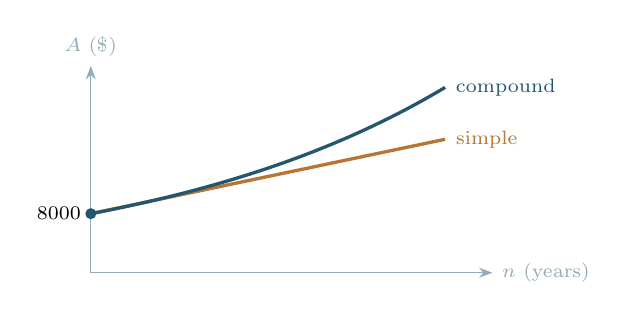
\begin{tikzpicture}[figstyle,x=0.75cm,y=0.75cm]
  \draw[chalkdk!50,->](0,0)--(6.8,0)node[right,font=\scriptsize]{$n$ (years)};
  \draw[chalkdk!50,->](0,0)--(0,3.5)node[above,font=\scriptsize]{$A$ (\$)};
  \draw[amber!85!black,very thick](0,1)--(6,2.26)node[right,font=\scriptsize]{simple};
  \draw[chalkdk,very thick,domain=0:6,samples=40,smooth]plot(\x,{1.21^\x})node[right,font=\scriptsize]{compound};
  \fill[chalkdk](0,1)circle(2pt);\node[left,font=\scriptsize]at(0,1){$8000$};
\end{tikzpicture}\end{center}

  \worklines{5}
  \end{hq}

  \item \begin{hq}Jai has \$10\,000 to invest for $3$ years. Option A pays $6\%$ p.a. compounded annually; Option B pays $5.8\%$ p.a. compounded monthly. Calculate the final amount for each option and state which is better.

  \worklines{6}
  \end{hq}

\end{enumerate}\clearpage

\sectionband{3I}{Introducing logarithms}{CORE}

\begin{refbox}
{\bfseries\color{chalkdk}Textbook worked examples}\;\textcolor{inksoft}{\small(cross-reference in your textbook)}\\[3pt]
\begin{itemize}[leftmargin=16pt,itemsep=1pt,topsep=2pt]
  \item \textbf{Example 24} --- Writing equivalent statements involving logarithms \textcolor{inksoft}{(p.\,268)}
  \item \textbf{Example 25} --- Evaluating logarithms \textcolor{inksoft}{(p.\,268)}
  \item \textbf{Example 26} --- Solving simple logarithmic equations \textcolor{inksoft}{(p.\,269)}
\end{itemize}
\vspace{4pt}{\bfseries\color{chalkdk}Question sets}\;\textcolor{inksoft}{\small(practise from your textbook)}\\[3pt]
\begin{itemize}[leftmargin=16pt,itemsep=1pt,topsep=2pt]
  \item \textbf{Building Understanding:} Q1--3 \textcolor{inksoft}{(p.\,268)}
  \item \textbf{Fluency:} Q1--5 \textcolor{inksoft}{(p.\,270)}
  \item \textbf{Problem-solving:} Q6--8 \textcolor{inksoft}{(p.\,270--271)}
  \item \textbf{Reasoning:} Q9--11 \textcolor{inksoft}{(p.\,271)}
  \item \textbf{Enrichment: Fractional logarithms:} Q12 \textcolor{inksoft}{(p.\,271)}
\end{itemize}\end{refbox}

\vspace{4pt}{\bfseries\color{chalkdk}\large Worked examples}\;\textcolor{inksoft}{\small(study the method, then try the hurdles)}\par

\begin{workedbox}

{\bfseries\color{chalkdk}Switching between index form and log form}\par\vspace{3pt}

\textbf{(a)} Write $3^4=81$ in logarithmic form. \textbf{(b)} Write $\log_2 32=5$ in index form.\par\vspace{2pt}

\figLogForm{3}{4}{81}

{\bfseries Solution.}\ $\log_a x=y$ and $a^y=x$ say the same thing: the base stays the base, and the log is the \textbf{power}. \[ \text{(a)}\;\; 3^4=81 \;\Leftrightarrow\; \log_3 81=4 \qquad\qquad \text{(b)}\;\; \log_2 32=5 \;\Leftrightarrow\; 2^5=32 \]

\end{workedbox}

\begin{workedbox}

{\bfseries\color{chalkdk}Evaluating logarithms and solving log equations}\par\vspace{3pt}

Evaluate \textbf{(a)} $\log_5 125$ and \textbf{(b)} $\log_{10} 0.001$ without a calculator. Then solve \textbf{(c)} $\log_3 x=4$ and \textbf{(d)} $\log_x 49=2$.\par\vspace{2pt}

{\bfseries Solution.}\ Read each log as the question ``\emph{base to what power gives the number?}'' Write equations in index form.\par\vspace{2pt}
\begin{tabular}{@{}l@{\quad}l}
\textbf{(a)} & $5^3=125$, so $\log_5 125=3$.\\[2pt]
\textbf{(b)} & $0.001=\tfrac{1}{1000}=10^{-3}$, so $\log_{10}0.001=-3$.\\[2pt]
\textbf{(c)} & $\log_3 x=4$ means $x=3^4$, so $x=81$.\\[2pt]
\textbf{(d)} & $\log_x 49=2$ means $x^2=49$, so $x=7$ (a base must be positive).
\end{tabular}

\end{workedbox}
\newpage
\vspace{6pt}{\bfseries\color{amber}\large Hurdle questions --- Section 3I}\;\textcolor{inksoft}{\small(show all working)}\par\nopagebreak\vspace{2pt}

\begin{enumerate}[leftmargin=20pt,itemsep=8pt,topsep=4pt,beginpenalty=10000,label=\textbf{H\arabic*.}]

  \item \begin{hq}Write each statement in \textbf{logarithmic form}: \textbf{(a)} $2^6=64$, \textbf{(b)} $10^4=10\,000$, \textbf{(c)} $5^{-2}=\tfrac{1}{25}$.

\figLogForm{a}{y}{x}

  \worklines{3}
  \end{hq}

  \item \begin{hq}Write each statement in \textbf{index form}: \textbf{(a)} $\log_3 243=5$, \textbf{(b)} $\log_{10}0.01=-2$, \textbf{(c)} $\log_6 1=0$.

  \worklines{3}
  \end{hq}

  \item \begin{hq}Evaluate without a calculator: \textbf{(a)} $\log_2 128$, \textbf{(b)} $\log_{10}100\,000$, \textbf{(c)} $\log_4\tfrac{1}{16}$.

  \worklines{4}
  \end{hq}

  \item \begin{hq}Solve for $x$: \textbf{(a)} $\log_5 x=3$, \textbf{(b)} $\log_x 64=3$, \textbf{(c)} $\log_7 x=0$.

  \worklines{4}
  \end{hq}

  \item \begin{hq}Use your calculator to evaluate $\log_{10}50$, correct to three decimal places. Then explain, using powers of $10$, why the answer must lie between $1$ and $2$.

\begin{center}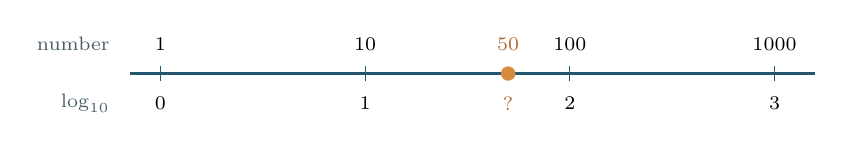
\begin{tikzpicture}[figstyle,x=2.6cm,y=1cm]
  \draw[chalkdk,thick](-0.15,0)--(3.2,0);
  \foreach \k/\n in {0/1,1/10,2/100,3/1000}{\draw[chalkdk](\k,-0.1)--(\k,0.1);\node[above=2pt,font=\scriptsize]at(\k,0.1){$\n$};\node[below=2pt,font=\scriptsize]at(\k,-0.1){$\k$};}
  \node[font=\scriptsize,inksoft,anchor=east]at(-0.2,0.38){number};\node[font=\scriptsize,inksoft,anchor=east]at(-0.2,-0.38){$\log_{10}$};
  \fill[amber](1.699,0)circle(2.6pt);\node[above=2pt,font=\scriptsize,amber!80!black]at(1.699,0.1){$50$};\node[below=2pt,font=\scriptsize,amber!80!black]at(1.699,-0.1){$?$};
\end{tikzpicture}\end{center}

  \worklines{3}
  \end{hq}

\end{enumerate}\clearpage

\sectionband{3J}{Logarithmic scales}{CORE}

\begin{refbox}
{\bfseries\color{chalkdk}Textbook worked examples}\;\textcolor{inksoft}{\small(cross-reference in your textbook)}\\[3pt]
\begin{itemize}[leftmargin=16pt,itemsep=1pt,topsep=2pt]
  \item \textbf{Example 27} --- Interpreting a logarithmic chart \textcolor{inksoft}{(p.\,276)}
  \item \textbf{Example 28} --- Constructing a logarithmic graph \textcolor{inksoft}{(p.\,278)}
\end{itemize}
\vspace{4pt}{\bfseries\color{chalkdk}Question sets}\;\textcolor{inksoft}{\small(practise from your textbook)}\\[3pt]
\begin{itemize}[leftmargin=16pt,itemsep=1pt,topsep=2pt]
  \item \textbf{Building Understanding:} Q1--2 \textcolor{inksoft}{(p.\,275--276)}
  \item \textbf{Fluency:} Q1--5 \textcolor{inksoft}{(p.\,279--280)}
  \item \textbf{Problem-solving:} Q6--8 \textcolor{inksoft}{(p.\,281--282)}
  \item \textbf{Reasoning:} Q9--11 \textcolor{inksoft}{(p.\,282--283)}
  \item \textbf{Enrichment: Exploring pH:} Q12 \textcolor{inksoft}{(p.\,283)}
\end{itemize}\end{refbox}

\vspace{4pt}{\bfseries\color{chalkdk}\large Worked examples}\;\textcolor{inksoft}{\small(study the method, then try the hurdles)}\par

\begin{workedbox}

{\bfseries\color{chalkdk}Reading a logarithmic chart}\par\vspace{3pt}

The chart shows $\log_{10}P$, where $P$ is the population of five towns. \textbf{(a)} What is the difference in order of magnitude between town A and town D? \textbf{(b)} How many times larger is the population of town A than town D?\par\vspace{2pt}

\figLogBars{A/5,B/3,C/4,D/2,E/6}{$\log_{10}P$}{6}

{\bfseries Solution.}\ The height of each bar is the \textbf{order of magnitude} (the power of $10$). \textbf{(a)} $5-2=3$. \textbf{(b)} Each step on a log scale multiplies by $10$, so a difference of $3$ means $10^3=1000$. Town A's population is \textbf{$1000$ times} larger than town D's.

\end{workedbox}

\begin{workedbox}

{\bfseries\color{chalkdk}Constructing a logarithmic graph}\par\vspace{3pt}

A culture of bacteria has $P$ cells after $t$ hours. Find $\log_{10}P$ for each value (one decimal place), plot $\log_{10}P$ against $t$, and describe the relationship.\par\vspace{2pt}

\begin{center}\renewcommand{\arraystretch}{1.25}\begin{tabular}{c|ccccc}
$t$ & $0$ & $1$ & $2$ & $3$ & $4$\\\hline
$P$ & $30$ & $300$ & $3000$ & $30\,000$ & $300\,000$\\
$\log_{10}P$ & $1.5$ & $2.5$ & $3.5$ & $4.5$ & $5.5$
\end{tabular}\end{center}

\loggrid{4}{6}{$\log_{10}P$}{$t$ (hours)}{\draw[chalkdk,thick](0,1.5)--(4,5.5);\foreach \t/\v in {0/1.5,1/2.5,2/3.5,3/4.5,4/5.5}{\fill[amber](\t,\v)circle(2.4pt);}}

{\bfseries Solution.}\ For example $\log_{10}30=1.477\ldots\approx1.5$. Each hour $P$ is multiplied by $10$, so $\log_{10}P$ goes up by exactly $1$. The points lie on a \textbf{straight line}, which tells us the relationship between $P$ and $t$ is \textbf{exponential}.

\end{workedbox}
\newpage
\vspace{6pt}{\bfseries\color{amber}\large Hurdle questions --- Section 3J}\;\textcolor{inksoft}{\small(show all working)}\par\nopagebreak\vspace{2pt}

\begin{enumerate}[leftmargin=20pt,itemsep=8pt,topsep=4pt,beginpenalty=10000,label=\textbf{H\arabic*.}]

  \item \begin{hq}The chart shows $\log_{10}R$, where $R$ is the yearly revenue (in dollars) of five companies. How many times larger is the revenue of: \textbf{(a)} company A than company C, \textbf{(b)} company D than company B, \textbf{(c)} company B than company E? \emph{(Part (c) is not a whole number of steps --- use your calculator, to one decimal place.)}

\figLogBars{A/6,B/4,C/3,D/5,E/2.5}{$\log_{10}R$}{6}

  \worklines{3}
  \end{hq}

  \item \begin{hq}An earthquake measures $7.2$ on the Richter scale and its aftershock measures $5.2$. \textbf{(a)} How many times more powerful was the main earthquake? \textbf{(b)} A later tremor was $1000$ times less powerful than the main earthquake. What did it measure?

\figLogLine{0}{9}{7.2}{main}{5.2}{aftershock}{Richter magnitude}

  \worklines{3}
  \end{hq}

  \item \begin{hq}On the pH scale, a \emph{lower} pH means more acidic, and each step is a factor of $10$. Vinegar has pH $3$ and pure water has pH $7$. \textbf{(a)} How many times more acidic is vinegar than water? \textbf{(b)} A soft drink is $100$ times more acidic than water. What is its pH?

\figLogLine{0}{14}{3}{vinegar}{7}{water}{pH}

  \worklines{4}
  \end{hq}

  \item \begin{hq}State the order of magnitude of \textbf{(a)} $3\,400\,000$ and \textbf{(b)} $0.0052$. \textbf{(c)} How many orders of magnitude larger is $3\,400\,000$ than $34$, and how many times larger is that?

  \worklines{5}
  \end{hq}

  \item \begin{hq}A population of insects is counted every hour. Complete the table (one decimal place), plot $\log_{10}A$ against $t$ on the grid, and describe what the graph tells you about the relationship between $A$ and $t$.

\begin{center}\renewcommand{\arraystretch}{1.35}\begin{tabular}{c|ccccc}
$t$ & $0$ & $1$ & $2$ & $3$ & $4$\\\hline
$A$ & $200$ & $600$ & $1800$ & $5400$ & $16\,200$\\
$\log_{10}A$ & \phantom{0.0} & \phantom{0.0} & \phantom{0.0} & \phantom{0.0} & \phantom{0.0}
\end{tabular}\end{center}

\loggrid{4}{5}{$\log_{10}A$}{$t$ (hours)}{}

  \worklines{3}
  \end{hq}

\end{enumerate}\clearpage

\sectionband{3K}{Laws of logarithms}{10A}

\begin{refbox}
{\bfseries\color{chalkdk}Textbook worked examples}\;\textcolor{inksoft}{\small(cross-reference in your textbook)}\\[3pt]
\begin{itemize}[leftmargin=16pt,itemsep=1pt,topsep=2pt]
  \item \textbf{Example 29} --- Simplifying logarithmic expressions \textcolor{inksoft}{(p.\,286)}
  \item \textbf{Example 30} --- Evaluating logarithmic expressions \textcolor{inksoft}{(p.\,286)}
\end{itemize}
\vspace{4pt}{\bfseries\color{chalkdk}Question sets}\;\textcolor{inksoft}{\small(practise from your textbook)}\\[3pt]
\begin{itemize}[leftmargin=16pt,itemsep=1pt,topsep=2pt]
  \item \textbf{Building Understanding:} Q1--3 \textcolor{inksoft}{(p.\,285)}
  \item \textbf{Fluency:} Q1--4 \textcolor{inksoft}{(p.\,287)}
  \item \textbf{Problem-solving:} Q5--7 \textcolor{inksoft}{(p.\,287)}
  \item \textbf{Reasoning:} Q8--10 \textcolor{inksoft}{(p.\,288)}
  \item \textbf{Enrichment: Proving the laws for logarithms:} Q11 \textcolor{inksoft}{(p.\,288)}
\end{itemize}\end{refbox}

\vspace{4pt}{\bfseries\color{chalkdk}\large Worked examples}\;\textcolor{inksoft}{\small(study the method, then try the hurdles)}\par

\begin{workedbox}

{\bfseries\color{chalkdk}Simplifying to a single logarithm}\par\vspace{3pt}

Write each as a single logarithm: \textbf{(a)} $\log_3 5+\log_3 4$, \textbf{(b)} $\log_2 36-\log_2 4$, \textbf{(c)} $3\log_5 2$.\par\vspace{2pt}

\begin{center}\renewcommand{\arraystretch}{1.3}\begin{tabular}{l@{\qquad}l@{\qquad}l}
\textcolor{inksoft}{\small Index law} & \textcolor{inksoft}{\small Log law} & \textcolor{inksoft}{\small In words}\\\hline
$a^m\times a^n=a^{m+n}$ & $\log_a x+\log_a y=\log_a(xy)$ & add logs $\leftrightarrow$ multiply numbers\\
$a^m\div a^n=a^{m-n}$ & $\log_a x-\log_a y=\log_a\!\left(\tfrac{x}{y}\right)$ & subtract logs $\leftrightarrow$ divide numbers\\
$(a^m)^n=a^{mn}$ & $\log_a x^n=n\log_a x$ & a coefficient $\leftrightarrow$ a power
\end{tabular}\end{center}

{\bfseries Solution.}\ Use one law per line, and name it. \begin{align*} \text{(a)}\;\;&\log_3 5+\log_3 4=\log_3(5\times4)=\log_3 20 &&(\text{addition law})\\ \text{(b)}\;\;&\log_2 36-\log_2 4=\log_2(36\div4)=\log_2 9 &&(\text{subtraction law})\\ \text{(c)}\;\;&3\log_5 2=\log_5 2^3=\log_5 8 &&(\text{power law}) \end{align*}

\end{workedbox}

\begin{workedbox}

{\bfseries\color{chalkdk}Combining logs, then evaluating}\par\vspace{3pt}

Evaluate without a calculator: \textbf{(a)} $\log_6 4+\log_6 9$, \textbf{(b)} $\log_3 54-\log_3 2$, \textbf{(c)} $2\log_{10}5+\log_{10}4$.\par\vspace{2pt}

{\bfseries Solution.}\ Combine into a single log first, then ask ``what power?'' \begin{align*} \text{(a)}\;\;&\log_6 4+\log_6 9=\log_6 36=2 &&(6^2=36)\\ \text{(b)}\;\;&\log_3 54-\log_3 2=\log_3 27=3 &&(3^3=27)\\ \text{(c)}\;\;&2\log_{10}5+\log_{10}4=\log_{10}25+\log_{10}4=\log_{10}100=2 &&(10^2=100) \end{align*}

\end{workedbox}
\newpage
\vspace{6pt}{\bfseries\color{amber}\large Hurdle questions --- Section 3K}\;\textcolor{inksoft}{\small(show all working)}\par\nopagebreak\vspace{2pt}

\begin{enumerate}[leftmargin=20pt,itemsep=8pt,topsep=4pt,beginpenalty=10000,label=\textbf{H\arabic*.}]

  \item \begin{hq}Write each as a single logarithm: \textbf{(a)} $\log_7 3+\log_7 5$, \textbf{(b)} $\log_{10}48-\log_{10}6$, \textbf{(c)} $4\log_2 3$.

  \worklines{4}
  \end{hq}

  \item \begin{hq}Evaluate without a calculator: \textbf{(a)} $\log_{10}20+\log_{10}5$, \textbf{(b)} $\log_2 96-\log_2 3$, \textbf{(c)} $\log_3 3^7$.

  \worklines{4}
  \end{hq}

  \item \begin{hq}Evaluate without a calculator: \textbf{(a)} $2\log_{10}2+\log_{10}25$, \textbf{(b)} $3\log_4 2+\log_4 8$. \emph{(Hint: use the power law first.)}

  \worklines{4}
  \end{hq}

  \item \begin{hq}Write $\log_5 50+\log_5 10-\log_5 4$ as a single logarithm, then evaluate it.

  \worklines{4}
  \end{hq}

  \item \begin{hq}Sam writes $\log_{10}(20+80)=\log_{10}20+\log_{10}80$. Show that Sam is wrong by evaluating both sides (use your calculator for the right-hand side, to three decimal places). Then write the correct law that Sam was trying to use.

  \worklines{4}
  \end{hq}

\end{enumerate}\clearpage

\sectionband{3L}{Solving exponential equations using logarithms}{10A}

\begin{refbox}
{\bfseries\color{chalkdk}Textbook worked examples}\;\textcolor{inksoft}{\small(cross-reference in your textbook)}\\[3pt]
\begin{itemize}[leftmargin=16pt,itemsep=1pt,topsep=2pt]
  \item \textbf{Example 31} --- Solving using the given base \textcolor{inksoft}{(p.\,290)}
  \item \textbf{Example 32} --- Solving using base 10 \textcolor{inksoft}{(p.\,290)}
\end{itemize}
\vspace{4pt}{\bfseries\color{chalkdk}Question sets}\;\textcolor{inksoft}{\small(practise from your textbook)}\\[3pt]
\begin{itemize}[leftmargin=16pt,itemsep=1pt,topsep=2pt]
  \item \textbf{Building Understanding:} Q1--3 \textcolor{inksoft}{(p.\,290)}
  \item \textbf{Fluency:} Q1--3 \textcolor{inksoft}{(p.\,291)}
  \item \textbf{Problem-solving:} Q4--6 \textcolor{inksoft}{(p.\,291--292)}
  \item \textbf{Reasoning:} Q7--9 \textcolor{inksoft}{(p.\,292)}
  \item \textbf{Enrichment: Change of base formula:} Q10 \textcolor{inksoft}{(p.\,292)}
\end{itemize}\end{refbox}

\vspace{4pt}{\bfseries\color{chalkdk}\large Worked examples}\;\textcolor{inksoft}{\small(study the method, then try the hurdles)}\par

\begin{workedbox}

{\bfseries\color{chalkdk}Solving $a^x=b$ with logarithms}\par\vspace{3pt}

Solve $5^x=40$. Give the exact answer and the answer correct to three decimal places.\par\vspace{2pt}

\figIntersect{5}{40}{$y=5^x$}{$x\approx2.292$}

{\bfseries Solution.}\ $x$ is in the power and $40$ is not a whole power of $5$, so use logs. In log form, $x=\log_5 40$ (exact). With base $10$ on the calculator, take $\log_{10}$ of both sides and use the power law: \[ x\log_{10}5=\log_{10}40 \;\Rightarrow\; x=\frac{\log_{10}40}{\log_{10}5}=\frac{1.60206}{0.69897}=2.292\ \text{(3 dp).} \] \emph{Check:} $5^2=25$ and $5^3=125$, so $x$ should lie between $2$ and $3$. \checkmark

\end{workedbox}

\begin{workedbox}

{\bfseries\color{chalkdk}Solving for time in a growth problem}\par\vspace{3pt}

\$2000 is invested at $6\%$ p.a., compounded annually, so $A=2000(1.06)^n$. After how many years will the investment first be worth at least \$5000?\par\vspace{2pt}

\figGrowth{$2000$}{$A=2000(1.06)^n$}{$n$ (years)}{$A$ (\$)}{\growthtarget{$5000$}{$n=\,?$}{2.5}}

{\bfseries Solution.}\ Set up the equation, isolate the power, then take $\log_{10}$ of both sides. \begin{align*} 2000(1.06)^n&=5000 \;\Rightarrow\; 1.06^n=2.5\\ n\log_{10}1.06&=\log_{10}2.5 \;\Rightarrow\; n=\frac{\log_{10}2.5}{\log_{10}1.06}=\frac{0.39794}{0.02531}=15.73 \end{align*} Interest is added once a year, so the investment first reaches \$5000 after \textbf{16 years}.

\end{workedbox}
\newpage
\vspace{6pt}{\bfseries\color{amber}\large Hurdle questions --- Section 3L}\;\textcolor{inksoft}{\small(show all working)}\par\nopagebreak\vspace{2pt}

\begin{enumerate}[leftmargin=20pt,itemsep=8pt,topsep=4pt,beginpenalty=10000,label=\textbf{H\arabic*.}]

  \item \begin{hq}Solve each equation, giving the exact answer as a logarithm and the answer correct to three decimal places: \textbf{(a)} $2^x=11$, \textbf{(b)} $3^x=100$.

\figIntersect{2}{11}{$y=2^x$}{$x=\,?$}

  \worklines{4}
  \end{hq}

  \item \begin{hq}Solve using base $10$, correct to three decimal places: \textbf{(a)} $7^x=300$, \textbf{(b)} $0.8^x=0.2$.

  \worklines{5}
  \end{hq}

  \item \begin{hq}A pond is stocked with $300$ fish, and the population grows by $5\%$ per month, so $P=300(1.05)^t$. Find the number of whole months until the population first reaches $750$.

\figGrowth{$300$}{$P=300(1.05)^t$}{$t$ (months)}{$P$}{\growthtarget{$750$}{$t=\,?$}{2.5}}

  \worklines{4}
  \end{hq}

  \item \begin{hq}A car worth \$40\,000 loses $12\%$ of its value each year. After how many whole years is it first worth less than \$10\,000?

\figDecay{$40\,000$}{$V=40\,000(0.88)^n$}{$n$ (years)}{$V$ (\$)}{\decaytarget{$10\,000$}{$n=\,?$}{0.25}}

  \worklines{4}
  \end{hq}

  \item \begin{hq}An $80$ g sample of a radioactive substance decays by $6\%$ every hour. Its \emph{half-life} is the time taken for half of it ($40$ g) to remain. Find the half-life, correct to two decimal places.

\figDecay{$80$}{$M=80(0.94)^t$}{$t$ (hours)}{$M$ (g)}{\decaytarget{$40$}{$t=\,?$}{0.5}}

  \worklines{5}
  \end{hq}

\end{enumerate}

\vfill
\begin{center}\small\color{inksoft}\rule{0.5\linewidth}{0.3pt}\\[3pt]
End of Chapter 3F--3L hurdle booklet --- check your working against the worked examples and ask in class if any hurdle question is unclear.
\end{center}
\end{document}
